\chapter{Eclipse ICE Tutorial Installation Details}
You have been provided a USB stick with all you will need for this tutorial. On
this drive is the following: ICE binaries for your OS, VisIt binaries for your
OS, tools to install Docker, all tutorial documentation and slides for today,
data files for the tutorial, and a Eclipse ICE workspace with ICE cloned for
your convenience. 

\section*{Docker Installation}
Before we begin, we will need to have Docker installed to enable scientific code
execution with ICE. ICE handles local and remote job launching for general
scientific computing, but since we don't have enough time in this tutorial to
build any science codes and their dependencies, we are providing a Docker image
with a science code already built and configured. To use it, you must have
Docker installed, which is OS specific. To see how to install Docker for your
OS, go to \url{https://docs.docker.com/engine/installation/}. For Linux this
is pretty self-explanatory, just use your package manager to install docker
and start the docker daemon running. 

For Mac and Windows users in this tutorial,
we have provided the Docker Toolbox installers on the USB stick. After
installing Docker Toolbox, you will need to start up a new docker machine. To do so, run the following:
\begin{lstlisting}[language=bash]
docker-machine create --driver virtualbox default
\end{lstlisting}
then on Mac OS, add the following to your bash\_profile
\begin{lstlisting}[language=bash]
eval "$(docker-machine env default)"
\end{lstlisting}
On Windows, you will need to run the following after creating the default
docker-machine:
\begin{lstlisting}[language=bash]
docker-machine env --shell cmd default
for /f "tokens=*" %i in ('docker-machine env 
		--shell cmd default') do %i
\end{lstlisting}

\section*{Starting ICE}
To start ICE, select the correct ice-product* zip file on the USB stick and
unzip it to get the ICE Application. Double-click to open up ICE. When the workspace chooser
dialog opens, select the workspace we have provided on the USB stick (either to
the location you copied it to on your local machine, or on the USB stick
itself, see below image). 
\begin{center} 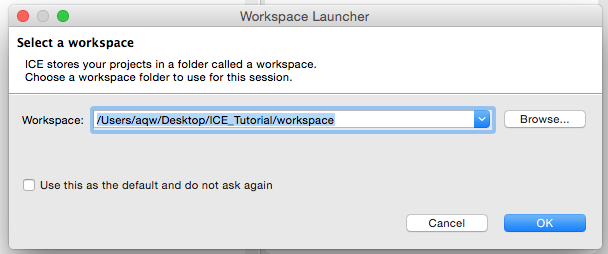
\includegraphics[width=\textwidth]{figures/workspace}
\end{center}
When ICE opens you should see something similar to the below image. 
\begin{center} 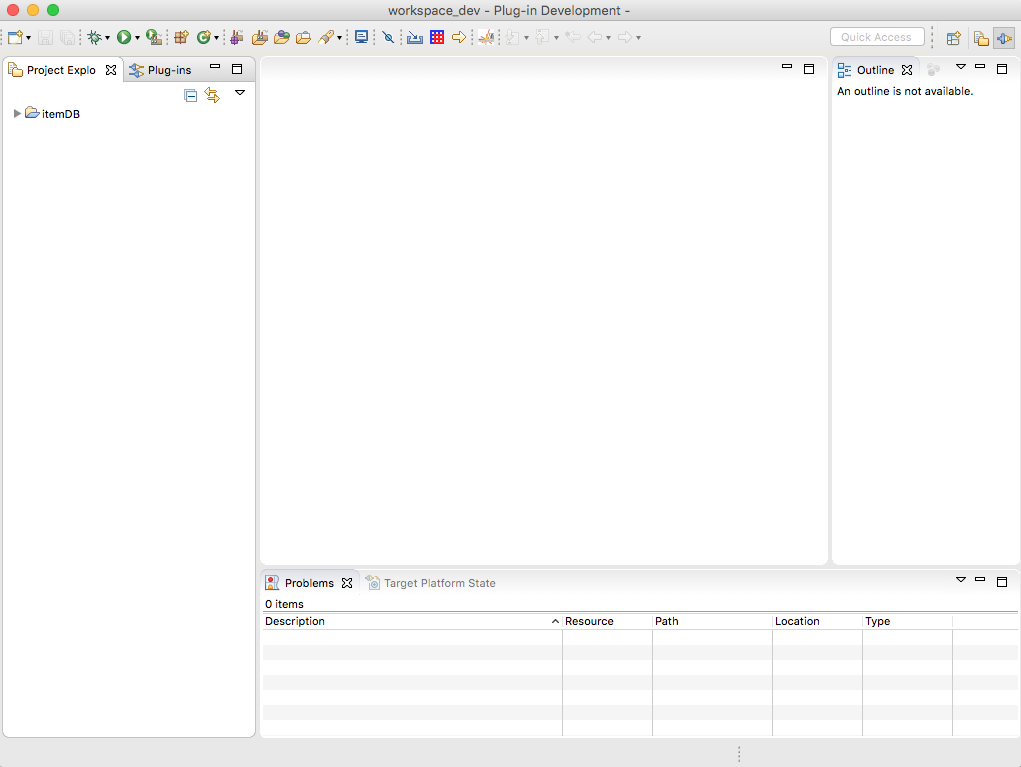
\includegraphics[width=\textwidth]{figures/expectedICE}
\end{center} 

The first thing you should do is import the existing projects in the workspace
we have provided. To do this, first open the Git perspective and select Add and
Existing Local Git Repository. Point the wizard to the ice folder in the
workspace, and import ICE as a new Git repository (you should have something
like the image below).
\begin{center} 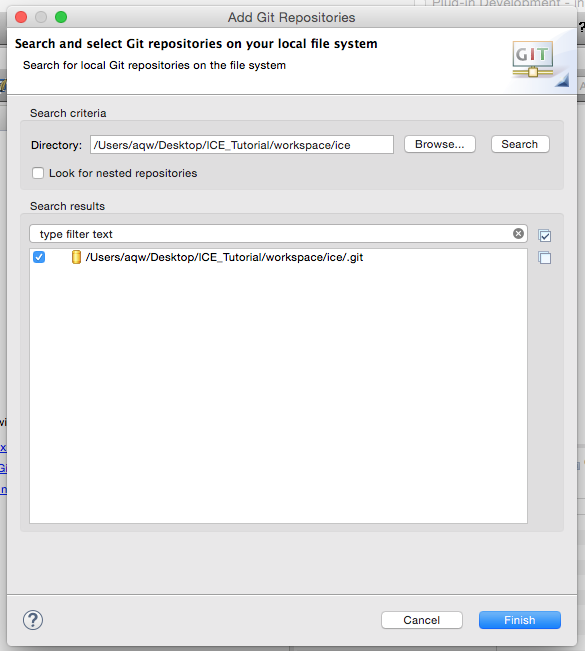
\includegraphics[width=\textwidth]{figures/clone} \end{center}
Now, right click on the ICE repository and select Import Projects. You should
see the below wizard pages, simply select Next on the first page, and Finish on
the second page.
\begin{center} 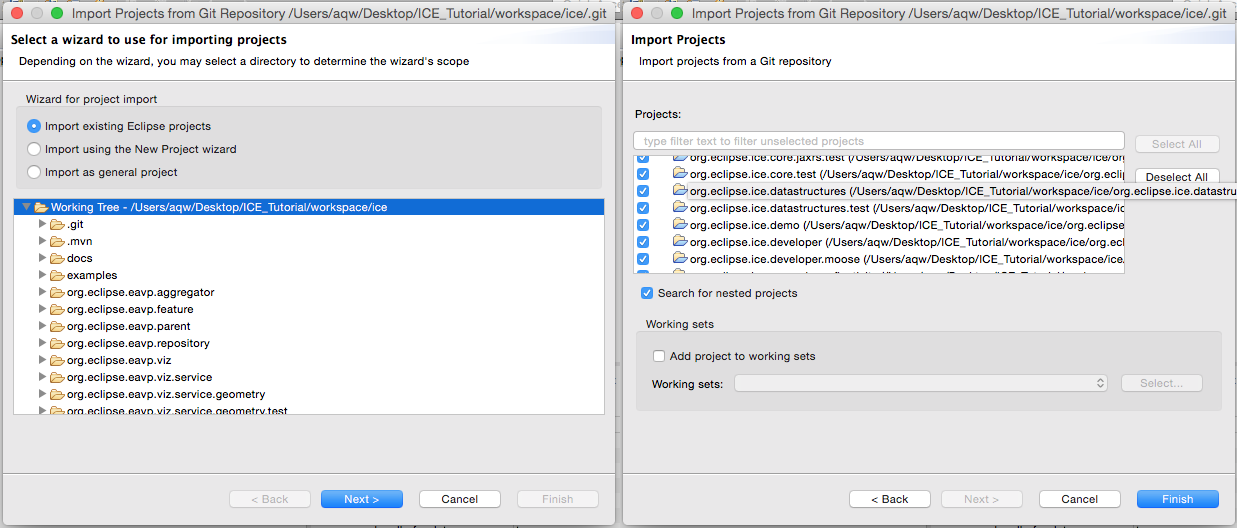
\includegraphics[width=\textwidth]{figures/importProjects}
\end{center}
After this you should see the following:
\begin{center} 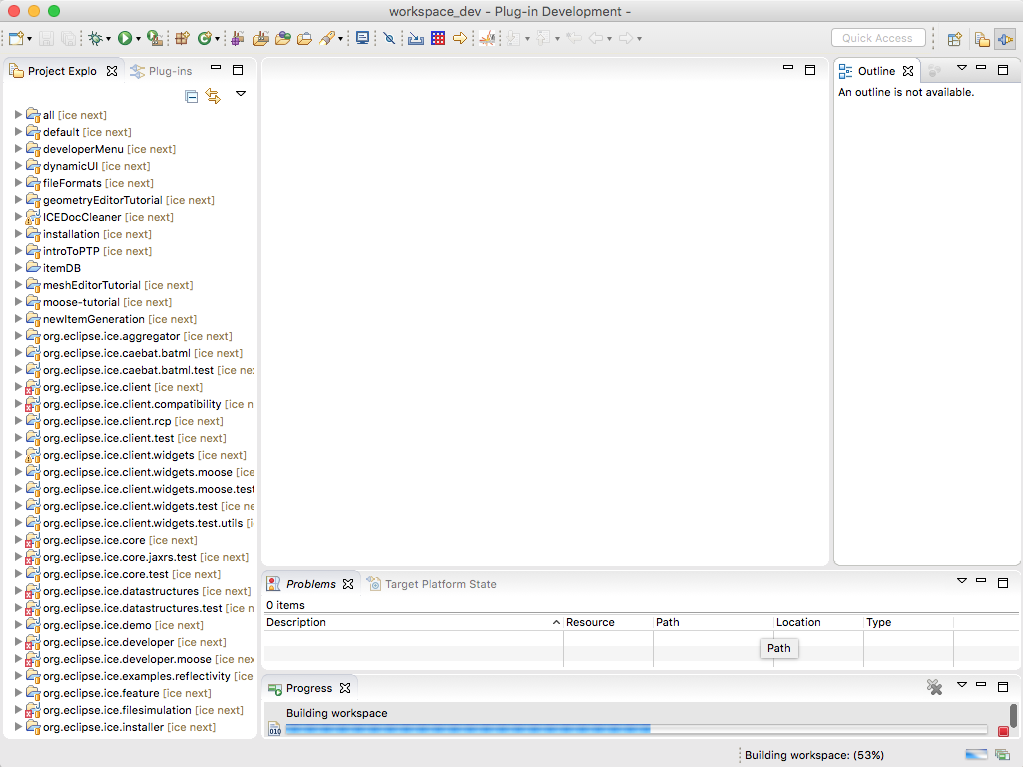
\includegraphics[width=\textwidth]{figures/cloned} \end{center}
